\documentclass[a4paper, top=10mm]{article}
%for writing from the top
\usepackage{fullpage}
%for math
\usepackage{amsmath}
\usepackage{mathrsfs}
\usepackage{amsthm}
%for images
\usepackage{graphicx}
%for color
\usepackage{xcolor}
%for title
\title{\textbf{\huge{Santa's Broken Stick}}}
\author{Enigma n\textsuperscript{o}2}
\date{19\textsuperscript{th} December 2024}

\newtheorem*{hint}{Hint}

\addtolength{\voffset}{-2cm}
\addtolength{\textheight}{5cm}


\begin{document}
	\maketitle
	
	Santa Claus, being very old and wise, always carries a trusty 1.6-meter stick to help him on his long journeys. One frosty evening, as he strolled through the workshop, disaster struck—the stick broke into two pieces!
	
	The oldest elf, quick on his feet, picked up the smaller of the two pieces and decided to use it as his own walking stick.
	
	On average, what is the length of the elf’s new stick?
	
	\textit{Provide your answer in millimeters, rounded to the nearest integer.}
	
	(Don’t worry—Santa was gifted a brand-new stick, custom-made by the elves!)
	
	\begin{center}
		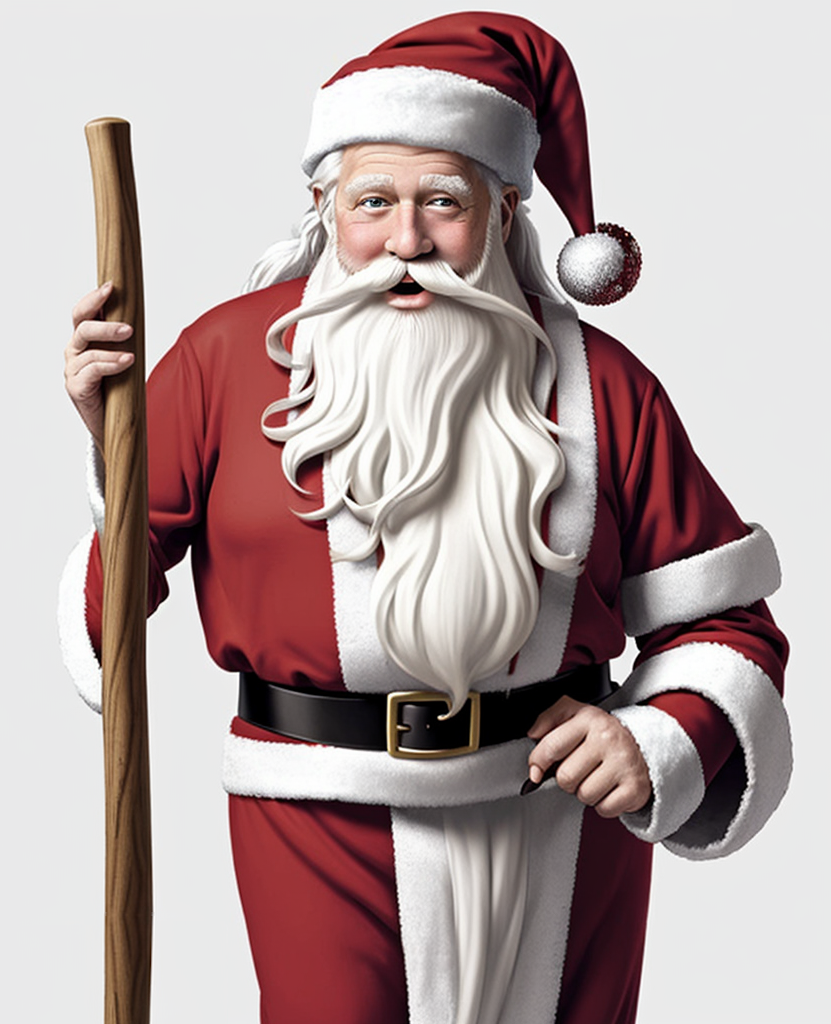
\includegraphics[height=400pt]{02santa_with_stick.png}\\
		Santa with his stick.
	\end{center}
	
	\underline{Note:} Suppose the breaking point follows a uniform probability law along the stick
	
	% Answer:
	% 400 mm
	% the smaller piece will uniformly random range from 0cm to 80cm => average 40cm
	
\end{document}